\chapter{Prize Collecting Partition}
\label{chapter:pc-partition}

This chapter aims to prove the Prize Collecting Partition Theorem (Theorem~\ref{theoremClustering}) presented below, allowing us to break a Steiner Multicycle instance into simpler, smaller ones. The proof relies upon an algorithm called Prize-Collecting Clustering, or PC-clustering, which will be presented later in this chapter.

\begin{theorem} \label{theoremClustering}
Given an \(\epsilon > 0\), a graph \(G_{in}\), a cost function associated with each edge in \(E(G_{in})\), and a set \(\mathcal{D}\) of terminal pairs, we can compute in polynomial time a set of disjoint components \(\{C_1, \dots, C_k\}\) (i.e., a set of subgraphs of \(G_{in}\)) with an associated partition of the set of terminal pairs \(\{\mathcal{D}_1, \dots, \mathcal{D}_k\}\) with the following properties:
\begin{enumerate}
    \item All demands are covered, that is, \(\mathcal{D} = \bigcup_{i=1}^k \mathcal{D}_i\); \label{condition_t_clust:1}
    \item All the terminals pairs in \(\mathcal{D}_i\) are covered by the component \(C_i\); \label{condition_t_clust:2}
    \item The sum of the cost of all the components \(C_i\) is no more than \((16/\epsilon + 4) \opt_{\mathcal{D}}(G_{in})\); \label{condition_t_clust:3}
    \item The sum of the costs of the minimum collection of cycles for each set of terminal pairs \(\mathcal{D}_i\) is no more than \(1 + \epsilon\) times the cost of a minimum solution of the SMCP in \(G_{in}\); that is, \(\sum_i \opt_{\mathcal{D}_i} (G_{in}) \leq (1 + \epsilon) \opt_{\mathcal{D}} (G_{in})\). \label{condition_t_clust:4}
\end{enumerate}
\end{theorem}

The last condition implies that we can solve the problem in each \(C_i\) separately and still guarantee an approximation with a small factor.

We start proving the Theorem~\ref{theoremClustering} by applying a 4-approximation algorithm in \(G_{in}\) (for instance, the algorithm for SMCP provided by \cite{Pereira2018TheSM}). Clearly, this construction satisfies the first two properties, since by definition an SMCP solution covers all demand sets, and for each set \(\mathcal{D}_i\) a component in the solution connects all of its terminals. To guarantee the last two properties, we need to employ the \textbf{PC-clustering} algorithm, which is presented in Section~\ref{section:pc_clustering}.

\section{Prize-Collecting Clustering} \label{section:pc_clustering}

The PC-Clustering algorithm is used in the proof of the following theorem - which by its turn will be used to prove Theorem~\ref{theoremClustering}. 
It is worth mentioning that the Theorem~\ref{theoremClustering_Bateni_3_1} is based on \cite{Bateni} (see Theorem 3.1 (Prize-Collecting Clustering)).

\begin{theorem} \label{theoremClustering_Bateni_3_1}
Let \(G=(V, E)\) be a graph with a nonnegative edge cost \(c(e)\) for each edge \(e\) and a potential \(\phi_v\) for each vertex \(v \in V\). 
There is a polynomial-time algorithm that computes a subgraph \(Z\) of \(G\) such that:

\begin{enumerate}
    \item the cost of \(Z\) is at most \(4 \sum \limits_{v \in V} \phi_v\), and \label{condition:1}
    \item \(Z\) is a spanning subgraph of \(G\), and \label{condition:2}
    \item all vertices in \(Z\) have even degree, and \label{condition:3}
    \item for any subgraph \(L\) of \(G\), there is a set  of vertices \(Q\) such that: \label{condition:4}
    \begin{enumerate}
        \item \(\sum \limits_{v \in Q} \phi_v\) is at most the cost of \(L\), and \label{condition:4a}
        \item if two vertices \(v_1, v_2 \notin Q\) are connected by \(L\), then they are  in the same component of \(Z\) \label{condition:4b}
    \end{enumerate}
\end{enumerate}
\end{theorem}

The statement above might look too abstract at first, but it will get more clear with its proof and application. First let us present a brief overview of the PC-Clustering algorithm, followed by a more complete description.

We start with a graph where vertices have associated potentials (or prizes) and edges have a crossing cost. The idea is to agglomerate the vertices into clusters progressively. 

Initially, each vertex induces an individual cluster. The total potential of a cluster equals the sum of the potentials of its internal vertices minus the cost of crossing its internal edges. At each step, clusters can use their potential to ``pay'' for crossing edges to merge with other clusters. That way, the algorithm iteratively spends the potential of the graph's vertices until all the potential is spent.

\citeauthor{Bateni} make an analogy to edge painting while presenting the algorithm, where each vertex is associated with a color, and its colors are used to paint edges to connect separated clusters; when an edge is fully painted, it merges two clusters.

To summarize, at the beginning of the algorithm, each vertex \(v\) of \(V\) has a potential \(\phi_v\) that can be spent in clusters that contain \(v\) (so this cluster can connect to other clusters to form new bigger clusters). We keep track of how much ``potential'' the vertex \(v\) spent on a cluster \(S\) via the variable \(\gamma_{S, v}\), where \(S \subseteq V: v \in S\). Given a cluster \(C\), we generalize the variable \(\gamma\) as \(\gamma_{C}:= \sum_{v \in C} \gamma_{C, v}\) to account for the total potential spent by any vertex in the cluster \(C\).

Note that, it is possible to derive a subgraph of \(G\) from \(\gamma\) by considering only the edges of \(G\) that met the Constraint~\eqref{ineq:1} on equality.

The algorithm consists of two stages: \textit{growth} and \textit{pruning}. At the growth stage, we aim to find a subgraph \(F_1\) and a corresponding \(\gamma\). Next, we \textit{prune} (i.e., remove) some of the edges of \(F_1\) to get another subgraph \(F_2\). And finally, we duplicate all edges in \(F_2\) to obtain \(M_2\).

Noticeably, the following inequalities must be respected throughout the whole process.

\begin{align}
&&\sum_{S\subseteq V: e \in \delta(S)} \sum_{v \in S} \gamma_{S, v} \leq c(e) && \forall e \in E \label{ineq:1} \\
&&\sum_{S \subseteq V: S \ni v} \gamma_{S, v} \leq \phi_v && \forall v \in V \label{ineq:2} \\
&&\gamma_{S, v} \geq 0 && \forall S \subseteq V, v \in S \label{ineq:3}
\end{align}

The main goal of the growth stage is to build a spanning subgraph \(F_1\) that partitions the vertices of \(G\). The intuition is to think of \(\phi_v\) as an amount of potential that \(v\) can spend in a cluster \(S\), to which it belongs (i.e., \(v \in S\)), to merge \(S\) with other clusters in \(G\). However, that must be done in a way that the total spent to cross an edge is no more than the cost of that edge (Constraint~\eqref{ineq:1}), and that vertex \(v\) of \(S\) does not use more potential than it has available (Constraint~\eqref{ineq:2}). The Constraint~\eqref{ineq:3} ensures that the value that \(v\) contributes to \(S\) is never negative.

We begin the growth stage with an empty \(\gamma\) (i.e., \(\forall v \in V\) and \(\forall S \subseteq V\) we have \(\gamma_{v, S} = 0\)) and a subgraph \(F_1\) also empty (i.e., has no edges). During this step, we keep track of a set of clusters \(\mathcal{C}\) which partitions the vertices of \(V(G)\); initially, each cluster is composed of a single vertex. We say that a cluster \(C \in \mathcal{C}\) is active if  \(\sum_{C' \subseteq C} \sum_{v \in C'} \gamma_{C', v} < \sum_{v \in C} \phi_v\) (i.e. the cluster \(C\) still has vertices with remaining potential). Notice that if a vertex \(v \in C_1 \subset C_2\) spent \(\gamma_{C_1, v}\) to join \(C_1\) with another cluster to form \(C_2\), the potential \(\gamma_{C_1, v}\) used cannot be used in \(C_2\).
As for clusters, we say that a vertex is active if it still has some spending potential.

During the growth process, we iteratively spend potential from vertices to grow all active clusters by an \(\eta\) value - which may vary between iterations. It is important to note that an equal amount of \(\eta\) is spent on each cluster within the same iteration, and for each cluster, each of its active vertices spends the same amount of potential. Thus, it is possible for the amount spent between vertices of different clusters to be different, depending on the number of active vertices in each cluster.

Let us consider a specific cluster \(C\) and denote \(\kappa(C)\) as the number of active vertices in \(C\). Each active vertex in \(C\) spends \(\eta / \kappa(C)\) of its available potential into the cluster \(C\). This implies that a total of \(\eta\) will be spent on \(C\) during the iteration.
The value of \(\eta\) is the largest possible value that still adheres to the constraints mentioned above (Constraints~\eqref{ineq:1}, \eqref{ineq:2} and \eqref{ineq:3}) for all active clusters.

After each growth iteration, some restrictions might reach equality. If the Constraint~\eqref{ineq:2} becomes tight for some vertices, then those vertices become inactive. 
If all vertices inside a cluster become inactive, then we say that the cluster itself becomes inactive. 
In case Constraint~\eqref{ineq:1} becomes tight for some edge \(uv\), then the potential spent by two neighboring clusters was enough to cover the cost of the edge. This implies that there are two clusters \(C_u \ni u\) and \(C_v \ni v\) which we can merge into a new cluster \(C = C_u \cup C_v\), by adding \(uv\) to \(F_1\). We then add the new cluster and remove the two former clusters from \(\mathcal{C}\).

Note that after each growth iteration, at least one of the restrictions will meet equality for some set of vertices and/or edges. Thus, after a polynomial number of iterations, either all restrictions are met in equality, or the potential of all vertices is spent.

The pruning stage iteratively removes some edges from \(F_1\) to form \(F_2\). This process is necessary for proving Lemma~\ref{clustering_connecting_bateni_3_4}. Let \(\mathcal{S}\) be the set containing all sets that were a cluster at some point during the growth stage. It can be easily observed that the clusters \(\mathcal{S}\) are laminar and the maximal clusters are the clusters of \(\mathcal{C}\). Note that \(F_1[C]\) is connected for each \(C \in \mathcal{S}\).

Let \(\mathcal{B} \subseteq \mathcal{S}\) be the set of all tight clusters at the end of the growth stage, i.e., for each \(S \in \mathcal{B}\) we have \(\sum_{S' \subseteq S} \sum_{v \in S'} \gamma_{S', v} = \sum_{v \in S} \phi_v\). At the start of the stage, we initialize \(F_2\) as \(F_1\). While there is a cluster \(S \in \mathcal{B}\) such that \(F_2 \cap \delta(S) = \{e\}\) (notice that if \(F_2 \cap \delta(S)\) has more than one edge we do not prune \(S\)), we remove the edge \(e\) from \(F_2\).

At the end of this process, \(F_2\) does not have edges of \(\delta(C)\); in other words, no connected component of \(F_2\) can have two vertices such that one belongs to \(C\) and the other does not.

For the Algorithm~\ref{algorithm:pc-clustering}, we define \(\mathcal{C}(v)\) as the cluster currently containing the vertex \(v \in V'\), that is, \(\mathcal{C}(v):= C\) for any \(v \in C \in \mathcal{C}\).

\begin{algorithm}[H]
\caption{PC-Clustering}
\label{algorithm:pc-clustering}
\begin{algorithmic}[1]

\Require Graph \(G(V , E)\), and potentials \(\phi_v > 0\).
\Ensure Subgraph \(M_2\).

\State Let \(F_1 \gets (V_{in}, \emptyset)\).
\State Let \(\gamma_{S, v} \gets 0\) for any \(S \subseteq V : v \in S\).
\State Let \(\mathcal{S} \gets \mathcal{C} \gets \{\{v\}: v \in V\}\).
\While {there is an active vertex} \label{alg:line-while}
    \State Let \(\eta\) be the largest possible value such that simultaneously increasing \(\gamma_C\) by \(\eta\) for all active clusters \(C\) does not violate Constraints \eqref{ineq:1}, \eqref{ineq:2} and \eqref{ineq:3}.
    \State Let \(\gamma_{\mathcal{C}(v), v} \gets \gamma_{\mathcal{C}(v), v} + \frac{\eta}{\kappa(\mathcal{C}(v))}\) for all active vertices \(v\).
    \If {\(\exists e \in E\) that is tight and connects two clusters}
        \State Pick one such edge \(e = (u, v)\).
        \State Let \(F_1 \gets F_1 \cup \{e\}\).
        \State Let \(C \gets \mathcal{C}(u) \cup \mathcal{C}(v)\).
        \State Let \(\mathcal{C} \gets \mathcal{C} \cup \{C\} \backslash \{ \mathcal{C}(u), \mathcal{C}(v) \}\).
        \State Let \(\mathcal{S} \gets \mathcal{S} \cup \{C\}\).
    \EndIf
\EndWhile

\State Let \(F_2 \gets F_1\).
\State Let \(\mathcal{B} \gets \{S \in \mathcal{S} : \sum_{S' \subseteq S} \sum_{v \in S'} \gamma_{S', v} = \sum_{v \in S} \phi_v\}\).
\While {\(\exists S \in \mathcal{B}\) such that \(F_2 \cap \delta(S) = \{e\}\) for an edge \(e\)}
    \State Let \(F_2 \gets F_2 \backslash \{e\}\).
\EndWhile
\State Duplicate edges of \(F_2\) to form \(M_2\).
\State Output \(M_2\).

\end{algorithmic}
\end{algorithm}

\begin{lemma}[\cite{Bateni} - Lemma 3.3] \label{clustering_bound_bateni_3_3}
    The cost of \(F_2\) is at most \(2 \sum_{v \in V} \phi_v\).
\end{lemma}
\begin{proof}
The PC-Clustering algorithm has a notion of time. At each discrete step of the algorithm (i.e., at each iteration of line~\ref{alg:line-while}), one of two events happens: a cluster becomes inactive, or an edge becomes tight. We call the ``time'' between two event points \textbf{epochs}. 

Notice that, during each epoch, each cluster is either active or inactive, and each active cluster \(C\) increases its \(\gamma_C\) value, while all other \(\gamma\)'s remain unchanged. At time \(0\), all (singleton) clusters with a strictly positive penalty are active.

We aim at proving that the cost of \(F_2\) is at most \(2 \sum_{S \subseteq V : v \in S} \gamma_{S, v} \leq 2 \sum_{v \in V} \phi_v\), where the inequality follows from Constraint~\eqref{ineq:2}.

Let \(t_j\) be the time at which the \(j^{th}\) event point occurs in the growth step. So the \(j^{th}\) epoch is the time interval between \(t_{j-1}\) to \(t_j\). For each cluster \(C\) let \(\gamma_{C}^{(j)}\) be the amount \(\gamma_{C}:= \sum_{v \in C} \gamma_{C, v}\) that the cluster grew during epoch \(j\), which is  \(t_j - t_{j-1}\) if it was active during this epoch, or zero otherwise. Thus, \(\gamma_C = \sum_j \gamma_C^{(j)}\).

Since each edge \(e\) of \(F_2\) was added at some point by the growth stage when its edge packing Constraint~\eqref{ineq:1} became tight, we can exactly apportion the cost \(c(e)\) amongst the collection of clusters \(\{K: e \in \delta(K)\}\) whose variables ``paid for'' the edge, and can divide this up further by epoch. In other words, \(c(e) = \sum_j \sum_{K : e \in \delta (K)} \gamma_K^{(j)}\). Summing over the epochs yields the desired conclusion.

We will now prove that, for an arbitrary epoch \(j\), the total edge cost of \(F_2\) that is apportioned from epoch \(j\) is at most \(2 \sum_C \gamma_C^{(j)}\). In other words, the total rate at which all active clusters pay for edges of \(F_2\) is at most twice the available potential of the active clusters during the epoch.

Let \(\mathcal{C}_j\) be the set of clusters that existed during epoch \(j\) (either active or inactive). Consider the graph \(F_2\) and then collapse each cluster \(C \in \mathcal{C}_j\) into a supernode. Let \(H\) be the resulting graph. We will continue to refer to each supernode as a ``cluster'' during the rest of the proof. Let us denote the active and inactive clusters in \(\mathcal{C}_j\) by \(\mathcal{C}_{act}\) and \(\mathcal{C}_{dead}\), respectively.

The edges of \(F_2\) that are being partially paid during epoch \(j\) are exactly those edges of \(H\) that are incident to an active cluster - and the total amount of these edges that are being paid during epoch \(j\) is \((t_j - t_{j - 1}) \sum_{C \in \mathcal{C}_{act}} deg_H(C)\). Since every active cluster grows by exactly \(t_j - t_{j - 1}\) in epoch \(j\), we have:

$$\sum_C \gamma_C^{(J)} \geq \sum_{C \in \mathcal{C}_j} \gamma_C^{(J)} = (t_j - t_{j - 1}) |\mathcal{C}_{act}|$$

Now we show that \(\sum_{C \in \mathcal{C}_{act}} deg_H(C) \leq 2|\mathcal{C}_{act}|\).

Since each cluster induces a connected subtree of \(F_1\) and \(H\) is built from the contraction of edges of \(F_2\), it does not introduce new cycles, which implies that \(H\) is a forest. 
Also, all the leaves in \(H\) must be active, because otherwise the corresponding cluster would have been pruned into another component during the pruning stage.

With this information about \(H\), it is easy to bound \(\sum_{C \in \mathcal{C}_{act}} deg_H(C)\). The total degree in \(H\) is at most \(2 (|\mathcal{C}_{act}| + |\mathcal{C}_{dead}|)\). Noticing that the degree of dead clusters is at least two, we get \(\sum_{C \in \mathcal{C}_{act}} deg_H(C) \leq 2 (|\mathcal{C}_{act}| + |\mathcal{C}_{dead}|) - 2|\mathcal{C}_{dead}| = 2|\mathcal{C}_{act}|\) as desired.

Finally, we obtain the following inequality because $t_j-t_{j-1} \ge 0$:

$$(t_j - t_{j - 1}) \sum_{C \in \mathcal{C}_{act}} \mathrm{deg}_H(C) \leq 2 (t_j - t_{j - 1}) |\mathcal{C}_{act}|$$

Since the left-hand side of the inequality is the total amount being paid to edges of \(F_2\) during epoch \(j\), by summing through all epochs, we get:

$$c(F_2) \leq 2 \sum_j \sum_C \gamma_C^{(j)} = 2 \sum_{S \subseteq V : v \in S} \gamma_{S, v} \leq 2 \sum_{v \in V} \phi_v.$$

\end{proof}

Let \(M_2\) be the graph created by duplicating each edge on \(F_2\). Notice that all vertices in \(M_2\) have even degrees, and besides that \(c(M_2) \leq 4 \sum_{v \in V} \phi_v\), which is formalized in the following result.

\begin{corollary} \label{corollary_1}
The cost of the graph \(M_2\) is at most \(4 \sum_{v \in V} \phi_v\)
\end{corollary}
\begin{proof}
    The result follows immediately from Lemma~\ref{clustering_bound_bateni_3_3}.
\end{proof}

The following lemma due to~\cite{Bateni} gives a sufficient condition for two vertices that end up in the same component of \(F_2\).

\begin{lemma}[\cite{Bateni} - Lemma 3.4] \label{clustering_connecting_bateni_3_4}
    Two vertices \(u\) and \(v\) of \(V\) are connected in \(F_2\) if there exist clusters \(S, S'\) both containing \(u\) and \(v\) such that \(\gamma_{S, v} > 0\) and \(\gamma_{S', u} > 0\).
\end{lemma}
\begin{proof}

    The growth stage connects \(u\) and \(v\) since \(\gamma_{S, v} > 0\) and \(u, v \in S\). Consider the path \(P\) connecting \(u\) and \(v\) in \(F_1\). All the vertices of \(P\) are in \(S\) and \(S'\). For the sake of reaching a contradiction, suppose some edges of \(P\) are pruned. Let \(e\) be the first edge being pruned in \(P\). 

    Thus, there must be a cluster \(C \in \mathcal{B}\) which cuts \(e\) (i.e. \(C\) only contains one endpoint of the edge \(e\)); furthermore, \(\delta(C) \cap E(P) = \{e\}\), since \(e\) is the first edge pruned from \(P\). As \(C\) cuts \(e\), the laminarity of the clusters gives \(C \subset S, S'\).

    In addition, note that \(C\) contains precisely one endpoint of the path \(P\) (as opposed to precisely one endpoint of the edge \(e\)). This holds because \(C\) contained neither or both endpoints of \(P\), so the cluster \(C\) could not cut \(P\) at exactly one edge.

    Let us call the endpoint of \(P\) in this cluster \(v\). We then have \(\sum_{C' \subseteq C} \gamma_{C',v} = \phi_v\) because \(C\) is tight. However, as \(C\) is a \textit{proper} subset of \(S\), this contradicts with \(\gamma_{S, v} > 0\), proving that the supposition is false. The case when \(C\) contains \(u\) is symmetric.
\end{proof}

As mentioned before, \citeauthor{Bateni} associate a color to each vertex so that the vertex ``spends'' its color to fill the edges. Therefore, we say that a cluster \(H\) exhausts a vertex's \(v\) color, when \(\sum_{C \subseteq H} \gamma_{C, v} = \phi_v\). This analogy will be mentioned in the lemmas ahead.

\begin{lemma}[\cite{Bateni} Lemma 3.5] \label{clustering_bateni_3_5}
    If a subgraph \(H=(V, E')\) of \(G\) connects two vertices \(u, v\) from different components of \(F_2\), then \(H\) exhausts the ``color'' corresponding to at least one of \(u\) and \(v\).
\end{lemma}
\begin{proof}
    Given that \(H\) connects \(u\) and \(v\), suppose that \(H\) exhausts neither \(u\) nor \(v\): there is a set \(S\) containing \(u\) and a set \(S'\) containing \(v\) such that \(\gamma_{S, v} > 0\) and \(\gamma_{S', u} > 0\) and \(E' \cap \delta(S) = E' \cap \delta(S') = \emptyset\). Since \(H\) connects \(u\) and \(v\), this is only possible if \(u\) and \(v\) are both in \(S\) and \(S'\). By Lemma~\ref{clustering_connecting_bateni_3_4}, this implies that \(F_2\) connects \(u\) and \(v\), a contradiction.
\end{proof}

We can relate the cost of a subgraph to the potential value of the colors it exhausts.

\begin{lemma}[\cite{Bateni} Lemma 3.6] \label{clustering_bateni_3_6}
    Let \(Q\) be the set of colors exhausted by subgraph \(G'\) of \(G\). The cost of \(G'(V, E')\) is at least \(\sum_{v \in Q} \phi_v\).
\end{lemma}
\begin{proof}
    This is quite intuitive. Recall that vertices have associated ``colors'' which are used to ``color'' the edges of \(G\) during cluster growth. Consider a segment on edges corresponding to cluster \(S\) with color \(v\). At least one edge of \(G'\) passes through the cut \((S, \overline{S})\). Thus, a portion of the cost of \(G'\) can be charged from \(\gamma_{S, v}\). Hence, the total cost of the graph \(G'\) is at least as large as the total amount of colors paid for by \(Q\).
\end{proof}


\begin{proof}[Proof of Theorem~\ref{theoremClustering_Bateni_3_1}]
The subgraph \(Z\) is the graph \(M_2\), which corresponds to the forest \(F_2\) with duplicated edges, which already guarantees Condition~\eqref{condition:3}.

Condition~\eqref{condition:1} is given by Corollary~\ref{corollary_1}. 

To assert Condition~\eqref{condition:2}, we must observe that as a first step of the growth stage of the Algorithm~\ref{algorithm:pc-clustering} we initialize each vertex as an individual cluster.

For Condition~\eqref{condition:4}, let \(Q\) be the set of vertices exhausted by \(L\). Now conditions~\eqref{condition:4a} and \eqref{condition:4b} are proved by Lemma~\ref{clustering_bateni_3_6} and Lemma~\ref{clustering_bateni_3_5}, respectively.

\end{proof}

\section{Proof of PC-Partition Theorem}

The proof of the PC-Partition Theorem (Theorem~\ref{theoremClustering}) induces an algorithm that outputs a set of components of an input graph \(G_{in}\). Such an algorithm is presented next.

\begin{algorithm}[H]
\caption{PC-Partition}
\label{algorithm:pc-partition}
\begin{algorithmic}[1]

\Require Graph \(G_{in} = (V_{in}, E_{in})\), a set of weights associated with the edges in \(E_{in}\) and a set of terminal pairs \(\mathcal{D}\)
\Ensure Set of components \(\{C_i\}_{i=1}^k\); such that \(C_i\) covers the terminals in \(\mathcal{D}_i\)
\State Use the algorithm proposed by \cite{Pereira2018TheSM} to find a Steiner Multicycle 4-approximated \(M^\ast = \{C^\ast_1, \dots, C^\ast_k\}\) of \(\mathcal{D}\).
\State Contract each cycle \(C_i^\ast\) in order to create a new graph \(G = (V, E)\).
\State For every \(v \in V\), let \(\phi_v\) be equal to \(\frac{1}{\epsilon}\) times the cost of the cycle \(C_i^\ast\) that was contracted into \(v\), and \(0\) in case there is no such cycle.
\State Let \(M_2\) be the solution produced by the PC-Clustering algorithm on \(G\) and \(\phi_v\).
\State Build \(M\) from \(M_2\) by \emph{uncontracting} all cycles \(C_i^\ast\).
\State Return the set of components \(\{C_i\}_{i=1}^k\), with \(\mathcal{D}_i := \{(s, t) \in \mathcal{D}: s, t \in V(C_i)\}\).

\end{algorithmic}
\end{algorithm}

\begin{proof}[Proof of Theorem~\ref{theoremClustering}]

Let \(G\) be the graph resulting from the contraction of the components of the 4-approximation \(M^\ast\) (as shown in Algorithm~\ref{algorithm:pc-partition}). For each component \(C\) of \(M^\ast\) contracted, resulting in a vertex \(v\), we define a potential \(\phi_v := \frac{1}{\epsilon} \cdot c(C)\) if \(v\) is the result of the contraction of a component of \(M^\ast\) and zero otherwise. 

Let \(Z\) be the subgraph of \(G\) given by Theorem~\ref{theoremClustering_Bateni_3_1}. Let \(Z_{in}\) be the subgraph of \(G_{in}\) obtained from \(Z\) by uncontracting the components of \(M^\ast\) and adding \(M^\ast\) to \(Z_{in}\). Note that \(Z_{in}\) is a spanning subgraph of \(G_{in}\), since \(Z\) is a spanning subgraph of \(G\) (Condition~\eqref{condition:2}).

Considering that \(M^\ast\) is a valid solution, and each vertex in \(Z\) has an even degree (Condition~\eqref{condition:3}), we have that \(Z_{in}\) is a valid solution for the SMCP as well. Let \(\{C_1, \dots, C_k\}\) be the components of \(Z_{in}\), and let \(\mathcal{D}_1, \dots, \mathcal{D}_k\) be the set of demand pairs covered by those components. It is clear that \(Z_{in}\) satisfies the Conditions~\eqref{condition_t_clust:1} and \eqref{condition_t_clust:2}.

To prove that \(Z_{in}\) satisfies Condition~\eqref{condition_t_clust:3}, note that the cost of \(Z_{in}\) is the cost of \(M^\ast\) (which is at most \(4 \cdot \opt\)) plus the cost of \(Z\) (which by Theorem~\ref{theoremClustering_Bateni_3_1} is at most \( 4 \sum_{v \in V} \phi_v = \frac{4}{\epsilon} c(M^\ast) \leq \frac{16}{\epsilon} \opt \) by construction ).


\begin{figure}[H]
    \centering
% \tikzset{
%     every node/.style={
%         circle,
%         draw,
%         solid,
%         fill=black!50,
%         inner sep=0pt,
%         minimum width=4pt
%     }
% }
\begin{tikzpicture}[thick,scale=1.8,-,shorten >=2pt]

    \draw (0,0) node {} -- (1,1) [dashed] node {};
    \draw (2, 1.5) node {} -- (3,2) [dashed] node {};
    
    \draw (1,2) node {} -- (2, 1.5) [dashed] node {};

    \draw (3, 0.3) node {} -- (4,0) [dashed] node {};
    \draw (3, 0.3) node {} -- (4,-1) [dashed] node {};
    \draw (0,2) node {} -- (1,2) [dashed] node {};
    \draw (4,1) node {} -- (3, 0.3) [dashed] node {};


    \draw (1,1) node {} -- (2, 1.5) [red] node {};
    \draw (3.03,2) node {} -- (4.03,1) [red] node {};
    \draw (2.03, 1.5) node {} -- (2.03,0) [red] node {};   
    \draw (1,1.04) node {} -- (1,-0.26) [red] node {};
    \draw (1,-0.27) node {} -- (2,0.03) [red] node {};
    \draw (0.05,0) node {} -- (0.05,2) [red] node {};
    \draw (4.03,1) node {} -- (4.03,0) [red] node {};

    \draw  (0,2) node {} -- (1,1) [green] node {};
    \draw (0,0) node {} -- (1,-0.3) [green] node {};
    \draw (1,0.95) node {} -- (2, 1.45) [green] node {};
    \draw (2.97,2) node {} -- (3.98,1) [green] node {};
    \draw (1.97, 1.5) node {} -- (1.97,0) [green] node {};
    \draw (1,-0.33) node {} -- (2,-0.03) [green] node {};
    \draw (0,0) node {} -- (0,2) [green] node {};
    \draw (3.97,1) node {} -- (3.97,0) [green] node {};

    \Vertex[x=1, y=2, color=white]{A}
    \Vertex[x=4, y=1, color=white]{B}
    \Vertex[x=3, y=0.3, color=white]{C}
    \Vertex[x=4, y=-1, color=white]{D}

    \Vertex[x=0, y=2, label=$t_1$, color=white]{t_1}
    \Vertex[label=$t'_1$, color=white]{t_1'}

    \Vertex[x=1, y=1, label=$t_2$, color=white]{t_2}
    \Vertex[x=2, y=0, label=$t'_2$, color=white]{t_2'}

    \Vertex[x=1, y=-0.3, label=$t_3$, color=white]{t_3}
    \Vertex[x=2, y=1.5, label=$t'_3$, color=white]{t_3'}

    \Vertex[x=3, y=2, label=$t_4$, color=white]{t_4}
    \Vertex[x=4, y=0, label=$t'_4$, color=white]{t_4'}

\end{tikzpicture}

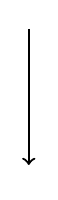
\begin{tikzpicture}[thick,scale=1.8,-,shorten >=2pt]
\draw[->, thick] (0,0) -- (0,-1);
\end{tikzpicture}

\begin{tikzpicture}[thick,scale=1.8,-,shorten >=2pt]

    \draw (0,-0.03) node {} -- (1,-0.03) [dashed] node {};
    \draw (0,0) node {} -- (0.5,1) [dashed] node {};
    \draw (1,0) node {} -- (0.5,1) [dashed] node {};

    \draw (1,0) node {} -- (2,1) [dashed] node {};
    % \draw (1,0) node {} -- (2,0) [dashed] node {};
    \draw (2,0) node {} -- (2,1) [dashed] node {};

    \draw (2,0) node {} -- (2.5,-0.5) [dashed] node {};


    \draw (0,0.03) node {} -- (1,0.03) [red] node {};

    \Vertex[x=0.5, y=1, color=white]{A}
    \Vertex[x=2, y=0, color=white]{B}
    \Vertex[x=2.5, y=-0.5, color=white]{C}

    \Vertex[x=0, y=0, label=$c_1$, color=white]{c_1}
    \Vertex[x=1, y=0, label=$c_2$, color=white]{c_2}
    \Vertex[x=2, y=1, label=$c_3$, color=white]{c_3}

\end{tikzpicture}

    \caption{In the top figure, the graph \(G\) is depicted with the approximated solution \(M\) and an optimal solution \(M^\ast\) represented with red and green lines, respectively. The bottom figure illustrates \(G\) contracted by \(M\), where each vertex \(\{c_1, c_2, c_3\}\) corresponds to a component of \(M\). The graph \(L\) consists of the red line and the vertices \(\{c_1, c_2, c_3\}\).}
    \label{fig:theorem_clustering_opt_contracted}
\end{figure}


Let \(Z_{in}^\ast\) be optimal solution for SMCP on \(G_{in}\), and let \(L\) be the subgraph of \(G\) corresponding to \(Z_{in}^\ast\) (obtained by contracting the components of \(M^\ast\)), as shown in Figure~\ref{fig:theorem_clustering_opt_contracted}. 

Let \(Q\) be the set of vertices of \(G\) given by the Condition~\eqref{condition:4} of Theorem~\ref{theoremClustering_Bateni_3_1}. The set \(Q\) might contain (or not) vertices from \(G\) that are a result of the contraction of components of \(M^\ast\). It is important to note that there is no need to compute \(Q\) and \(L\) to execute the algorithm. 

Let \(Q_{in}\) be the subgraph of \(G_{in}\) composed of the components of \(M^\ast\) whose contracted vertices in \(G\) belongs to \(Q\). From Condition~\eqref{condition:4a} of Theorem~\ref{theoremClustering_Bateni_3_1}, we have \(c(Q_{in}) = \epsilon \sum_{v \in Q} \phi_v \leq \epsilon c(L) \leq \epsilon \opt\).

To show that the last condition holds, for every \(\mathcal{D}_i\) (i.e., the set of demand pairs connected by \(C_i\)), we construct a subgraph \(H_i\) that satisfies the demands in \(\mathcal{D}_i\). Initially, \(H_i\) is empty. For each demand pair in \(\mathcal{D}_i\), if the component \(K\) of \(M^\ast\) that satisfies the demand belongs to \(Q_{in}\), then we add \(K\) to \(H_i\). Otherwise, we add the component of \(Z_{in}^\ast\) that satisfies the demand into \(H_i\). It is worth mentioning that the algorithm does not actually compute \(H_i\), because that would require to know \(Z_{in}^\ast\) and \(Q_{in}\).

Observe that each component of \(Q_{in}\) is used in at most one of the \(H_i\)’s: as \(Q_{in}\) is a subgraph of \(Z_{in}\), all the demands satisfied by a component \(K\) of \(Q_{in}\) belong to the same \(\mathcal{D}_i\).

Furthermore, we claim that each component of \(Z_{in}^\ast\) is used in at most one of the \(H_i\)'s. Suppose that a component \(K\) of \(Z_{in}^\ast\) was used in both \(H_i\) and \(H_j\), i.e., \(K\) satisfies a demand pair in \(\mathcal{D}_i\) and a demand pair in \(\mathcal{D}_j\). The components of \(M^\ast\) satisfying these two demands are not in \(Q_{in}\) (otherwise we would have put these components into \(H_i\) or \(H_j\) instead of \(K\)), thus they correspond to nodes \(v_1, v_2 \notin Q\) in the contracted graph \(G\). Thus \(L\), the contracted version of \(Z_{in}^\ast\), connects two nodes \(v_1, v_2 \notin Q\). In this situation, Condition~\eqref{condition:4b} of Theorem~\ref{theoremClustering_Bateni_3_1} implies that \(v_1\) and \(v_2\) are in the same component of \(Z\) and hence the two demands are satisfied by the same component of \(Z_{in}\). This contradicts that the two demands are in two different sets \(\mathcal{D}_i\) and \(\mathcal{D}_j\), since each component \(C_i\) of \(Z_{in}\) attends all demand pairs in each \(\mathcal{D}_i\).

Since every component of \(Q_{in}\) and every component of \(Z_{in}^\ast\) is used by at most one of the \(H_i\)'s, we have \(\sum_{i=1}^k c(H_i) \leq \opt + c(Q_{in}) \leq (1 + \epsilon) \opt\). Each \(H_i\) was constructed from components of \(Q_{in}\) and \(Z_{in}^\ast\), which establishes the last condition of the theorem.

\end{proof}
